% vim: textwidth=99 spell spelllang=en_gb:
% chktex-file 36

\documentclass[nobib, a4paper, twoside, justified]{tufte-book}

\usepackage[utf8]{inputenc}
\usepackage[british]{babel}
\usepackage{csquotes}
\usepackage[style=verbose, autocite=footnote, backend=biber]{biblatex}

\title{Displaying Heraldic\\Blazons}
\author{William Mathewson}
\publisher{University of Edinburgh}
\date{January 2018}

\addbibresource{bibliography.bib}

%%%%
%%
%% LOCALS are in `tufte-book-local.tex'

\usepackage{graphicx} % allow embedded images
\setkeys{Gin}{width=\linewidth,totalheight=\textheight,keepaspectratio}
\graphicspath{{graphics/}} % set of paths to search for images
\DeclareGraphicsExtensions{.pdf,.png}

\usepackage{amsmath}  % extended mathematics
\usepackage{booktabs} % book-quality tables
\usepackage{units}    % non-stacked fractions and better unit spacing
\usepackage{multicol} % multiple column layout facilities
\usepackage{fancyvrb} % extended verbatim environments
\usepackage{amsmath}
\usepackage{xspace}
\usepackage{makeidx}
\usepackage{mathtools}

\usepackage{float}
\usepackage{subfig}

\usepackage[final]{pdfpages}

%% Tell hyperref package it may break long URLs however it feels
\usepackage{hyperref}
\def\UrlBreaks{\do\/\do-}

%\newcommand{\dcim}{\emph{DCIM}\@\xspace}
%\newcommand{\ipam}{\emph{IPAM}\@\xspace}
%\newcommand{\dcimipam}{\emph{DCIM \& IPAM}\@\xspace}
%\newcommand{\desired}{\emph{desired}\@\xspace}
%\newcommand{\operational}{\emph{operational}\@\xspace}
%\newcommand{\wikid}{\textsc{WikiD}\@\xspace}
%\newcommand{\pywikid}{\textit{pywikid}\@\xspace}
\newcommand{\code}[1]{\texttt{#1}}
%\newcommand{\pythonthree}{Python$3$\@\xspace}

\newcommand{\svg}{\gls{svg}\@\xspace}
\newcommand{\svgs}{\glspl{svg}\@\xspace}
\newcommand{\dom}{\gls{dom}\@\xspace}

\newcommand{\charge}{\gls{charge}\@\xspace}
\newcommand{\charges}{\glspl{charge}\@\xspace}
\newcommand{\tincture}{\gls{tincture}\@\xspace}
\newcommand{\tinctures}{\glspl{tincture}\@\xspace}
\newcommand{\quarter}{\gls{quarter}\@\xspace}
\newcommand{\quarters}{\glspl{quarter}\@\xspace}

\newcommand{\blazon}{\gls{blazon}\@\xspace}
\newcommand{\blazons}{\glspl{blazon}\@\xspace}
\newcommand{\ublazon}{\Gls{blazon}\@\xspace}
\newcommand{\ublazons}{\Glspl{blazon}\@\xspace}

\newcommand{\payload}{\gls{payload}\@\xspace}
\newcommand{\payloads}{\glspl{payload}\@\xspace}

%\newcommand{\defeq}{\stackrel{\mathclap{\normalfont\mbox{def}}}{=}}
%\newcommand{\namedmap}[1]{\stackrel{\mathclap{\mbox{\small#1}}}{\longmapsto}}

%% R_{x->y} style
%\newcommand{\relate}[3]{\text{\itshape#1 }_{#2\ \mapsto\ #3}}

%% x --R--> y style
%\newcommand{\relate}[3]{#2\namedmap{#1}#3}

%% xRy style
%\newcommand{\relate}[3]{_{#2}#1_{#3}}

%\newcommand{\citetodo}{\sidenote{\todo{[Citation Needed]}}\@\xspace}
%\newcommand{\reftodo}{\sidenote{\todo{[Reference Needed]}}\@\xspace}
%\newcommand{\prooftodo}{\sidenote{\todo{[Substantiation Needed]}}\@\xspace}
\newcommand{\todo}[1]{{\noindent\textcolor{Red}{\textit{\quad#1}}\par}}

\let\lines\baselineskip{}

\usepackage{glossaries}
\setacronymstyle{long-short}

\loadglsentries{glossary}

\glstoctrue{}

\begin{document}

\frontmatter

\maketitlepage{}

%\abstract{This is an example of {\tt infthesis} style. The file {\tt
%skeleton.tex} generates this document and can be used to get a ``skeleton''
%for your thesis. The abstract should summarise your report and fit in the
%space on the first page.
%%
%You may, of course, use any other software to write your report, as long as
%you follow the same style. That means: producing a title page as given here,
%and including a table of contents and bibliography.  }

\begin{publicationmeta}
  \section*{Acknowledgements}
  I would like to thank my supervisor, Julian Bradfield, for his help and advice as I was writing
  this project. I would also like to thank all my friends on Level 9 of Appleton Tower,
  particularly Connie and Paul, who helped keep me going through the long, arduous journey that was
  this project and 4\textsuperscript{th} year as a whole.

  \section*{Declaration}
  I declare that this thesis was composed by myself,
  that the work contained herein is my own
  except where explicitly stated otherwise in the text,
  and that this work has not been submitted for any other degree or
  professional qualification except as specified.\par
  ({\textit{\thanklessauthor}})
\end{publicationmeta}

\tableofcontents

%\pagenumbering{Arabic}

\mainmatter{}

\chapter{Introduction}\label{cha:introduction}

This project was written as a paired project and as such I only wrote the side of the project that
deals with rendering the \blazons{}, having been parsed by the back end. The back-end was
written by my partner, Anthony Gallagher, and the writing of it will not be covered in this report.
Important shared design elements will be covered however in Section~\ref{sec:core_concepts}.

\section{Motivation}\label{sec:motivation}

In 1874 --- 4 years after his death --- John Papworth's \textit{Ordinary of British Armorials} was
published~\autocite{collins_1942}. In this work, he recorded approximately 50,000 entries of
descriptions of families' coats of arms, none annotated.

This honours project would make it possible to have these descriptions, or \textit{\blazons{}} as
they are termed in heraldry (see~\ref{sec:heraldry}), drawn freely for people to view. This has
potential application for ancestry companies that build family trees for people. Given the
\blazon{}, they would be able to construct the shields visually.

\section{Contributions}\label{sec:contributions}

In this honours project, my contributions included:

\begin{itemize}
  \item Drawing the \charges{} and \quarters{} used on the shield, or \textit{\gls{escutcheon}},
  \item Writing the base web server and
  \item Writing the \quarter{} and \charge{} drawing algorithm
\end{itemize}

\chapter{Background}\label{cha:background}

\section{Heraldry}\label{sec:heraldry}

Many families, countries and organisations --- primarily in Europe --- have coats of arms. Coats of
arms were initially used on shields on the battlefield to identify individual knights, but later
came to be used as flags and banners for individuals and families of the upper class at court. The
Royal Coat of Arms of the United Kingdom, belonging to the British monarch, can be seen in
Figure~\ref{fig:royal_coa}. If the reader wishes to learn more about Heraldry and its history, I
would recommend to you the many heraldic works of Charles Boutell and John Brooke-Little.

\begin{marginfigure}
  \centering
  \def\svgwidth{0.8\linewidth}
  \input{graphics/Royal_Coat_of_Arms_of_the_United_Kingdom.pdf_tex}
  \caption{The Royal Coat of Arms of the United Kingdom.
  Source:~\url{https://upload.wikimedia.org/wikipedia/commons/9/98/Royal_Coat_of_Arms_of_the_United_Kingdom.svg}}%
  \label{fig:royal_coa}
\end{marginfigure}

At the centre of a coat of arms is a shield known as an \textit{\gls{escutcheon}}. The language
used to describe how the escutcheon is to be drawn is known as a \textit{\blazon}.
\ublazons have been used since the Norman conquest and have been refined to a regular language
in the process~\autocite{boutell_1864}, although, as John Brooke-Little said, ``many of the
supposedly hard and fast rules laid down in heraldic manuals [including those by heralds] are often
ignored.''~\autocite{brooke_little_1985} This flagrant disregard for the rules introduces
difficulty in parsing the \blazons as the language loses some of its regularity.

\begin{marginfigure}
  \centering
  \def\svgwidth{0.8\linewidth}
  \input{graphics/Blason_Albert.pdf_tex}
  \caption{The shield of the town of Albert, France. \textit{Barry of ten argent and
  gules}. Source:~\url{https://en.wikipedia.org/wiki/File:Blason_Albert.svg}}%
  \label{fig:blason_albert}
\end{marginfigure}

\ublazons have a few key attributes:
\begin{itemize}
  \item The \textit{\gls{field}}, which is the background colour of the shield or
    \quarter{};
  \item \textit{\Glspl{ordinary}}, which are geometric shapes (as seen in Figure~\ref{fig:scrope},
    bearing a golden slash, or \textit{bend});
  \item \textit{\Glspl{charge}}, which are small emblems, such as fleur-de-lis and lions;
  \item \textit{\Glspl{variation}}, which describe how the field or \charge{} is patterned.
    \Glspl{variation} can indicate patterns such as chequered or coloured lines (as seen in
    Figure~\ref{fig:blason_albert}); and
  \item \textit{\Glspl{tincture}}, which are the colours and patterns for \charges{}, ordinaries
    and fields.
\end{itemize}

The tinctures are derived from Norman French and are divided into 3 groups, typically known as
\textit{metals}, \textit{colours} and \textit{furs}. In British heraldry, the colours are also
derived from Norman French and so the names appear archaic. In heraldry, blue is \textit{azure} and
red is \textit{gules} for instance. The metals are \textit{or} and \textit{argent}, for gold and
silver respectively. Whilst the tinctures are linked to colours, the College of Arms does not
specify which shade of that colour is required for the tinctures, leaving it to the artist to
decide~\autocite{college_of_arms_faq}. In this case, I have used default CSS colours.

\begin{marginfigure}
  \centering
  \def\svgwidth{0.8\linewidth}
  \input{graphics/chief_example.pdf_tex}
  \caption{\textit{Purpure, a chief Gules}.}%
  \label{fig:chief_example}
\end{marginfigure}

\ublazons conventionally follow a form of starting with the \textit{\gls{tincture}} or
\textit{\gls{variation}} of the field. After the description of the field,
\textit{\glspl{ordinary}} and \textit{\charges{}} are named with their tinctures. An example of
this is ``\textit{Purpure, a chief Gules}''. This \blazon describes an escutcheon with a field of
\textit{purpure} (purple), with a \textit{Chief} \gls{ordinary} --- a bar across the top of the
shield --- of \textit{gules} (red). This can be seen --- drawn by the web app --- in
Figure~\ref{fig:chief_example}.

\begin{marginfigure}
  \centering
  \def\svgwidth{0.8\linewidth}
  \input{graphics/scrope.pdf_tex}
  \caption{The Scrope \gls{escutcheon}; \textit{Azure, a bend Or}.}%
  \label{fig:scrope}
\end{marginfigure}

A simple --- but notable --- \blazon is that of the Scrope family. In the 14th century, the Baron
Scrope brought a case action against Sir Robert Grosvenor when he noticed that they both had the
same coat of arms. Many witnesses gave evidence in the case, including Geoffrey
Chaucer~\autocite{scrope_grosvenor}. The case was ultimately decided in Scrope's favour. The Scrope
coat of arms has a \blazon of \textit{Azure, a bend Or}; a depiction of this (as drawn by the web
app written for this project) can be seen in Figure~\ref{fig:scrope}.

Whilst the Scrope arms are prominent in heraldry, they are simplistic and indicative of
medi\ae{}val arms. Coats of arms became more complex as they developed through the centuries, with
instances of \textit{quarterly} shields, \textit{grand-quarterlies} --- quarterlies within
quarterlies --- and \textit{differenced} arms. \textit{Differenced} arms involve adding an
\textit{\gls{ordinary}} over an existing coat of arms. This was typically used to differentiate similar
looking coats of arms, especially between father and sons. Common examples of differentiated
shields are seen in duchies' coats of arms, particularly those which were given to Charles II's
illegitimate children. Examples of more complex shields can be seen in
Figure~\ref{fig:complex_shields}.

\begin{figure*}[h]
  \subfloat[Neville, 16th Earl of Warwick's coat of arms. An example of grand-quarterlies and
  differenced arms. Source:~\url{https://en.wikipedia.org/wiki/File:Neville_Warwick_Arms.svg}.]{%
    \def\svgwidth{0.3\linewidth} %
    \input{graphics/Neville_Warwick_Arms.pdf_tex}
  }
  \qquad
  \subfloat[A quarterly shield drawn by the web app. \textit{Quarterly: 1st and 4th: Gules, a bend
  Sable; 2nd and 3rd: Azure, a chief Or}. ]{%
    \def\svgwidth{0.28\linewidth}
    \input{graphics/quarterly_example.pdf_tex}
  }
  \caption{Some examples of more complex coats of arms.}\label{fig:complex_shields}
\end{figure*}

For a time, it was considered bad form to repeat a \textit{tincture} in a \blazon, and use a
reference to the tincture's previous use. The Heraldic Society gives an example as such:
``\textit{`Azure on a fess argent three billets azure'} [would have been written as] \textit{`Azure
on a fess argent three billets of the first'}''. The `\textit{of the first}' refers to the field's
tincture of azure. This \blazon describes a blue shield, with a white bar horizontally across the
middle with 3 white rectangles arranged along the bar. The Heraldic Society advocates repeating
tinctures to reduce ambiguity~\autocite{blazon_in_coa}.

\section{Related Works}%
\label{sec:related_works}

\todo{Add more related works}

Whilst many escutcheons have been drawn and uploaded to WikiMedia in
\svg~\autocite{ferraiolo2000scalable} format (some of which have been used in this report), many
appear to have been created in Inkscape~\autocite{inkscape}, rather than being created
programmatically. Much work has been done in collecting and cataloguing \blazons themselves ---
namely John Papworth as mentioned in Section~\ref{sec:motivation}.

\section{Summary}%
\label{sec:background_summary}

In this chapter, we covered basic heraldry, including core terminology, as well as works related to
the project. Core heraldry terminology includes:

\begin{itemize}
  \item \textit{\Gls{escutcheon}} --- the shield in the coat of arms;
  \item \textit{\Gls{field}} --- the background of the escutcheon;
  \item \textit{\Glspl{ordinary}} --- geometric shapes on the escutcheon;
  \item \textit{\Glspl{charge}} --- small emblems, such as fleur-de-lis and lions; and
  \item \textit{\Gls{tincture}} --- the colours and patterns for \charges{}, ordinaries and fields.
\end{itemize}

All relevant heraldry terminology may be found in the Glossary on page~\pageref{glossary}.

\chapter{Design}%
\label{cha:design}

\section{Core Concepts}%
\label{sec:core_concepts}

The two languages chosen for implementing this project were Python and
TypeScript~\autocite{typescript}. Python seemed like an obvious choice with its good support for
\gls{nlp} through the \gls{nltk}~\autocite{bird2004nltk}. TypeScript is a typed superset of
JavaScript written by Microsoft that compiles, or \textit{\glspl{transpile}}, to plain JavaScript.
TypeScript was chosen as a nicer alternative to programming in pure JavaScript, thanks to the
addition of powerful features such as types, access control and abstract classes. As a note to the
reader, to maintain interoperability with JavaScript, TypeScript uses trailing types, rather than
preceding types as in C. An example being that an \texttt{int} defined in C would be
\texttt{int~limit}, but in TypeScript, this would be \texttt{limit:~number}. (JavaScript/TypeScript
also has a unified \texttt{number} type to handle both \texttt{float}s and \texttt{int}s.)

The core design for this project centred around having a split stack; with a Python back-end
parsing the \blazon, serialising it into JSON \marginnote{\gls{json} is a lightweight
  data-interchange format, consisting of key-value pairs, array data types and other serialisable
  data types (such as strings, numbers and booleans). JSON is derived from JavaScript's associative
array-style data type, \texttt{Object}. An example of JSON can be seen in
Figure~\ref{fig:expected_output}.} and passing it to the TypeScript front-end, which then drew it
onto the webpage. This allowed for large amounts of flexibility, enabling the two halves of the
project to be developed in tandem with the Separation of Concerns principle being adhered to
throughout. It also allows for pluggable rendering implementations as the JSON schema for drawing
\payloads can be well-defined.

The Python back-end received a JSON \payload from the webpage containing the \blazon; it parsed the
\blazon using a Context-Free Grammar (CFG) parser and identified the most important parts of the
\blazon. It then serialised these back into a JSON response to be sent to the webpage for rendering.
The specification was such that if the webpage was given a \blazon of ``Azure, a bend Or'', it would
return the JSON \payload seen in Figure~\ref{fig:expected_output}.

\begin{figure}[h]
  \begin{verbatim}
    {
      "field": "azure",
      "charges": [{
        "charge": "bend",
        "tincture": "or"
      }]
    }
  \end{verbatim}
  \caption{Expected output from the Python back end, for a given \blazon of ``Azure, a bend Or''.}%
  \label{fig:expected_output}
\end{figure}

The TypeScript front-end received this \payload, applied the \textit{azure} CSS class to the field
element, then drew a bend onto the field with an \textit{or} CSS class.

Escutcheons were drawn using the \svg{} format for portability across browsers as well as the
eponymous scalability of \svg{} images. This allowed drawn escutcheons to be embedded elsewhere
with ease, either directly or through rendering the \svgs{} as other image formats via programmes
like Inkscape.

For version control, \texttt{git}~\autocite{git} was used and all code was hosted on GitHub.

\section{External Dependencies}%
\label{sec:external_dependencies}

The front-end depended on a pair of libraries for \svg{} rendering and \dom{} manipulation: the
selection library of D3.js~\autocite{d3js} and jQuery~\autocite{jquery}. D3.js provides many
powerful functions for \svg{} and \dom{} manipulation, especially creating and editing \svg{} and
HTML elements. It would also rely on jQuery for further \dom{} manipulation. The Mozilla Developer
Network defines the \dom{} as such: ``The \glsentryfirst{dom} connects web pages to scripts or
programming languages. Usually that means JavaScript, but modelling HTML, SVG, or XML documents as
objects is not part of the JavaScript language. The \dom{} model represents a document with a
logical tree. Each branch of the tree ends in a node, and each node contains objects.  \dom{}
methods allow programmatic access to the tree; with them you can change the document's structure,
style or content. Nodes can have event handlers attached to them. Once an event is triggered, the
event handlers get executed.''~\autocite{mdn_dom}.

For further assets, Sass~\autocite{sass-lang} was used as a CSS pre-processor and
Bootswatch~\autocite{bootswatch-flatly} was used for the base styling.  Webpack~\autocite{webpack}
was used to \gls{transpile} TypeScript down to JavaScript --- minifying and uglifying it in the
process --- and concatenate all source files and their dependencies into one main JavaScript
\textit{bundle} file. \textit{\Gls{minification}} of JavaScript assets involves stripping out all
unnecessary whitespace and tokens. \textit{\Gls{uglification}} transforms the JavaScript code by
renaming all variables and functions into short, obfuscated names to reduce the footprint of the
assets. These two techniques can decrease loading times of web apps as the browser have smaller
asset payloads to download than the original, raw source code.

\subsection{Development Dependencies}%
\label{sub:development_dependencies}

To maintain code readability and prevent bugs, TSLint~\autocite{tslint} was used and set up to
automatically run as part of the Travis \gls{ci}~\autocite{travis} service, causing a build to fail
if the linter detected a style violation. For unit testing, Jest~\autocite{jest} (with
ts-jest~\autocite{ts-jest} for TypeScript support) was used, especially for its powerful mocking
and expectation matcher functionality. Automated documentation generation was provided by
TypeDoc~\autocite{typedoc}.

\section{Iterative Design}%
\label{sec:iterative_design}

Iterative design was used as the design process for writing the code for this project. Iterative
design is a cyclical process of designing, prototyping and evaluating. One designs and prototypes a
new feature before evaluating the final feature design. If the design is acceptable, the new
feature is implemented, otherwise the cycle restarts. An iterative design process allows to address
different functionality as separate tasks, building on top of one another. It also allows to
heavily refactor a project whilst staying in one cycle.

\chapter{Implementation}%
\label{cha:implementation}

\section{Basic Charge Rendering}%
\label{sub:basic_charge_rendering}

\subsection{First Design Iteration}%
\label{sub:first_design_iteration}

The first design iteration had a specific focus on basic \charge{} drawing, with a plan to begin a
second iteration for adding quarterly rendering with lessons learnt from implementing \charge{}
drawing in the first iteration. The second design iteration is described in
Section~\ref{sub:second_design_iteration}.

I decided to have all drawing logic defined in the client, existing in a single module with minimum
dependencies. The shield outline was rendered on the page on load as part of the HTML template.
This helped support a reliable entry point for the drawing logic as it was able to easily select
the shield element to begin appending other \svg{} elements to. Appending these \svg{} elements
allowed layering to be achieved as \svg{} orders layers based on the order of elements in the
document. This was used to great effect later when drawing quarters (see
Section~\ref{sub:second_design_iteration}).

The front-end was designed around functional paradigms; breaking up major functionality into
functions that would deal with smaller, encapsulated functionality, such as adding extra layers to
the HTML template or clearing the shield when drawing a new \blazon. This allowed for a stable API,
as the single point of access function would not be renamed but all other functions may be changed
and updated separately. As described in Section~\ref{sec:core_concepts}, the front-end first
accessed the \textit{field} value in the parsed JSON \payload, applied the value as the CSS class
for the shield and then moved onto the \charges{}. It iterated over the \textit{\charges{}} array
in the \payload, drawing each \charge{} onto the shield and applying the tincture as the CSS class.
Due to \svg{} layering, as mentioned earlier, if there were multiple \charges{} specified in the
\payload, all would be drawn according to the array ordering.

\subsection{First Design Implementation}%
\label{sub:first_design_implementation}

As described in Section~\ref{sub:first_design_iteration}, the initial approach was to have all methods in
the core \texttt{index.ts} file that would be \gls{transpile}d and loaded in the browser. This
meant a smaller footprint when the code was bundled by Webpack and easier maintenance as all
relevant functions were next to one another, following the Step-Down
Rule~\autocite{martin2009clean}\footnote{The Step-Down Rule dictates that if function \texttt{A()}
calls function \texttt{B()} and \texttt{C()} in its function body, functions \texttt{A()} and
\texttt{B()} should be defined immediately after function \texttt{A()}.}.

\subsubsection{\texttt{drawShield(\blazon)}}%
\label{ssub:draw_shield}

The web app had a single entry point of \texttt{drawShield(\blazon)}, where \texttt{\blazon} was
the whole JSON \payload returned from the \texttt{/\_parse} endpoint. (See
Figure~\ref{fig:expected_output} for an example \payload.) This presented a problem initially as
TypeScript didn't handle the unstructured parsed data well due to it being a JavaScript
\texttt{Object}\footnote{In JavaScript, an \texttt{Object} works as both an associative array and a
basis for classes and inheritance through its \texttt{prototype} field.} instance. Attempting to
access members of this object (such as \texttt{\gls{field}}) causes TypeScript to produce an error
that the contents might be undefined and thus return a \texttt{null} object. To fix this, I
designed \texttt{interface}s with the expected fields in the \payload; one for the whole object,
\texttt{IBlazon}, and one for the \charges{} array contained within, \texttt{ICharge}. Similarly,
to avoid problems with string matching, I defined 2 \texttt{enum}s to represent the supported
tinctures and \charges{}, \texttt{ETincture} and \texttt{ECharge} respectively. As discussed in
Section~\ref{sec:adding_quarterly_rendering}, I later added another \texttt{enum} for quarters.
(All \texttt{interface}s and \texttt{enum}s can be found in
Appendix~\ref{cha:interfaces_and_enums}.) Having fixed this data problem,
\texttt{drawShield(\blazon)} was now able to access members of the \blazon object safely.

\subsubsection{\texttt{clearShield()}}%
\label{ssub:clear_shield}

To avoid the problem of overlapping \charges{}, I had to write a \texttt{clearShield()} method that
would iterate over all the \texttt{path} nodes in the \svg{} document, and delete them. This,
however, promptly deleted the shield outline, so I had to add a check to prevent deleting
\texttt{path} nodes with a \texttt{\#shield} id, instead only removing the CSS class. Having
cleared the shield of any possible obstructions, the \texttt{drawShield} method would then assign
the contents of the \texttt{field} value as the CSS class and iterate over the \texttt{\charges{}}
array, passing each \charge{} to \texttt{drawCharge(charge:~ICharge)}.

\subsubsection{\texttt{drawCharge()} and \texttt{ChargeShapes}}%
\label{ssub:draw_charge}

When each \charge{} node is created in \texttt{drawCharge}, it is assigned an id. This id is formed
from the name of the charge, followed by a random number in the range $1\text{--}512$ inclusive
with the hope that the range is large enough to lack overlaps.

To draw shapes in \svg{}, a \texttt{path} node requires a `\texttt{d}' attributes which contains
the commands for drawing said shape. To generate all these attributes, I drew all the \charge{}
shapes in Inkscape and extracted the `\texttt{d}' attribute from the generated \svgs{}. At first, I
put a \texttt{Map}\footnote{A \texttt{Map} here is a TypeScript/JavaScript data type, also known as
a \texttt{HashMap} or an associative array} of the \charges{} and their paths in the global scope,
available for all functions to access. This worked for \charges{} that were produced using a
\texttt{path} node with a `\texttt{d}' attribute, but introduced problems when using the
\textit{chief} \charge{} (a chief \charge{} being displayed in Figure~\ref{fig:chief_example}). The
chief \charge{} was drawn using a \texttt{rect} node which required `\texttt{x}' and `\texttt{y}'
co-ordinates to specify a starting point and \texttt{height} and \texttt{width} attributes to
describe the size of the rectangle. To address this, I wrote a \texttt{ChargeShapes} class to
encapsulate the \charges{} and their attributes. This class provided one public member,
\texttt{chargePaths} which was of the type \texttt{Map<string, Map<string, string>\hphantom{}>}.
Having this as a map allowed \texttt{drawCharge} to first check if the app knew how to draw the
\charge{} by checking whether \texttt{ChargeShapes.chargePaths} contained the \charge{} as a key.
If the \charge{} had an entry, then \texttt{drawCharge} would iterate over the attribute
\texttt{Map} and apply them to the \texttt{path} or \texttt{rect} node, before finally applying the
CSS class.

\begin{marginfigure}
  \centering
  \def\svgwidth{0.8\linewidth}
  \input{graphics/sinister_example.pdf_tex}
  \caption{\textit{Or, a bend sinister Vert.}}\label{fig:sinister_example}
\end{marginfigure}

The final part of \texttt{drawCharge} applied a transform to the \texttt{path} if the \payload
included a boolean flag \texttt{sinister} to indicate that the bend \charge{} should be flipped.
This writes to an attribute \texttt{transform} which applies a \texttt{matrix} transformation that
flips the \charge{} followed by a \texttt{translate} transformation to move it into place. An
example of a sinister bend can be seen in Figure~\ref{fig:sinister_example}.

\subsection{First Design Evaluation}%
\label{sub:first_design_evaluation}

Whilst this simple implementation worked well for drawing basic \glspl{escutcheon}, like
Figure~\ref{fig:chief_example} and Figure~\ref{fig:sinister_example}, it wasn't able to draw more
complex shields like those seen in Figure~\ref{fig:complex_shields}.

\section{Adding Quarterly Rendering}%
\label{sec:adding_quarterly_rendering}

\subsection{Second Design Iteration}%
\label{sub:second_design_iteration}

\subsubsection{Design Principles}%
\label{ssub:design_principles}

Whilst prototyping for adding functionality to render quarterly shields, I found that it was going
to be impossible to maintain the initial, atomic design laid out in
Section~\ref{sub:first_design_iteration} whilst also keeping the code clean and readable. This started the
second design iteration of the project. In this iteration, I designed a new, modular system that
leaned more heavily into Object-Oriented paradigms than functional ones. This new design was
written to follow the principles of delegation, decoupling, the Single
Responsibility~\autocite{martin2000design} and Open/Closed principles~\autocite{martin2000design}.

The Single Responsibility principle dictates that a class should have one, and only one, reason to
change. In \textit{Design Principles and Design Patterns}~\autocite{martin2000design}, Martin
defines a responsibility as a reason to change, such that a class should only change if that one
responsibility changes. If another responsibility is introduced, it should be given its own class.
This principle works well with decoupling as responsibilities can be changed in individual classes
without affecting other classes that use it. The Open/Closed principle dictates that a class should
be open to extension but closed to modification. A typical example of this would be using abstract
classes; the interface specified by the abstract class is closed to modification, but the child
classes may extend the functionality in their implementation. Thus, another class depending on the
class extending the abstract class can rely on the interface without having to know about the
internals.

To comply with these principles, all major sections of functionality, including \blazon
\payload parsing, \charge and \quarter rendering, were encapsulated in their own classes with clear
names and well-defined, shared APIs.

\subsubsection{Top-Level Design}%
\label{ssub:top_level_design}

The new design had a top-level class of \texttt{\ublazon} which had a single public function,
\texttt{draw()}. The \texttt{draw} method, as before, would clear the shield and then delegate
drawing responsibility to specialised \texttt{\charge{}} and \texttt{\quarter{}} renderers by
calling their \texttt{draw()} methods. This \texttt{\ublazon} class became the new entry-point,
being instantiated and called in a \texttt{main()} function in \texttt{index.ts}. In a similar
fashion to the top-level \texttt{\ublazon} class, a \texttt{\Gls{quarter}} class was defined to
enable proper delegation for rendering both the \quarter \textit{and} the \charges contained within
the quarter. The new \texttt{ChargeRenderer} class would contain most major logic for drawing, as
well as \texttt{id} generation. \texttt{QuarterRenderer} extended \texttt{ChargeRenderer} to add
\quarter-specific logic, while also being able to call up to it to draw the contained \charges.

For a quarterly \blazon, the \payload would have the \texttt{\gls{field}} value set to
\texttt{``quarterly''} and rather having a field \texttt{charges:~ICharge[]}, it would contain a
field \texttt{quarters:~IBlazon[]}. This worked as \quarters are treated as their own small
\glspl{escutcheon} in heraldry and are described as such. An example of a quarterly \blazon would
be \textit{Quarterly: 1st and 4th: Gules, a bend Sable; 2nd and 3rd: Azure, a chief Or}, as seen in
Figure~\ref{fig:complex_shields}. It was then possible to change functionality of the app depending
on the contents of the \texttt{field} key. To account for the new quarters that needed to be drawn,
a new \texttt{enum} \texttt{EQuarter} was designed, with the values of the enumerable options being
the \texttt{id}s of the \svg elements and the \texttt{path}s in the
\texttt{ChargeShapes.chargePaths} \texttt{Map}.

\subsubsection{Using \svgs for Great Good}%
\label{ssub:using_svg_for_great_good}

In this refactor, I also made use of more \svg properties: clip paths and the \texttt{<g>} element.
Clip paths allowed defining a path that cropped the element it was defined on. This was
particularly useful for drawing \charges inside of \quarters as the edges outside of the \quarter
would be cropped out by the clip path defined for that \quarter. The \texttt{<g>} element is a
grouping element for \svg; it applies all transformations defined on it to all its child elements
and any of its attributes are also inherited. I used the \texttt{<g>} elements for both grouping
together charges and quarters, but also explicitly named layers for the shield outline and the
\charges within.

\subsection{Second Design Implementation}%
\label{sub:second_design_implementation}

The Figure references in the following headings refer to the UML diagrams in
Appendix~\ref{sec:second_design_iteration_diagrams}.
%UML diagrams for all classes mentioned in this subsection can be found in
%Appendix~\ref{sec:second_design_iteration_diagrams}.

\subsubsection{\texttt{Blazon} (Figure~\ref{fig:BlazonUML})}%
\label{ssub:blazon}

\texttt{\ublazon} took 2 arguments in its \texttt{constructor}, \texttt{svg} and \texttt{data}.
\texttt{svg} was a D3.js~\autocite{d3js} data type that contained a selector for the \texttt{<svg>}
element in the HTML document, for appending elements to. The \texttt{data} argument was to take the
full JSON \payload returned by the parser. The \texttt{constructor} would then turn the
\texttt{data} \texttt{Object} into a \texttt{Map} object for more reliable access. To get more
fine-grained access to the \svg document, the \texttt{constructor} also populated extra fields with
selections of the whole shield element and the \texttt{<g id=``charge\_layers''>} element, defined
within the \texttt{svg} selection. The \texttt{chargesLayer} field is needed for telling the
renderer classes where to draw their shapes.  Depending on the contents of the \payload, the
\texttt{constructor} then instantiates new \texttt{ChargeRenderer} objects for all the
\texttt{\charges}, or instantiates 4 new \texttt{Quarter} objects for all the \quarters.

\texttt{clearShield} was also extracted from \texttt{index.ts} into \texttt{Blazon}, but with
changes to account for many \texttt{<path>} nodes as well as \texttt{<clipPath>} elements. The
method now iterated over both child elements of the \texttt{<g id=``charge\_layers''>} and
\texttt{<clipPaths>} with an \texttt{id} beginning with \texttt{``quarterly\_''}, deleting them in
the process. It also stripped the \texttt{shield} node of its CSS class.

\subsubsection{\texttt{Quarter} (Figure~\ref{fig:QuarterUML})}%
\label{ssub:quarter}

The new \texttt{Quarter} class relied on the order of the \texttt{quarters} array in the payload to
determine which quarter it was representing; with numbering starting at 0 in the top left quarter,
going left to right, ending at 3 in the bottom right. The \texttt{constructor} required the array
index as its first argument, with \texttt{field:~ETincture}, \texttt{charges:~ICharge[]},
\texttt{svg} and \texttt{chargesLayer} as its other arguments. With these parameters, the
\texttt{constructor} selected the quarter specified by the \texttt{index}, instantiated
\texttt{ChargeRenderer} objects --- borrowing a method from \texttt{Blazon} --- and a
\texttt{QuarterRenderer} object. The \texttt{draw()} method of \texttt{Quarter} first called the
\texttt{draw()} method on the \texttt{QuarterRenderer} object to draw the quarter \texttt{path}
onto the shield, then called \texttt{addClipPathDefinition(svg)} (see
Section~\ref{ssub:charge_renderer}) to add a new clip path to the \svg document. Having used
\texttt{QuarterRenderer} to draw a new quarter \texttt{path}, it selected it, assigned it to a
locally scoped constant, \texttt{quarterLayer}, and iterated over the \texttt{charges}. Before
calling the \texttt{draw} method on the \texttt{charge} object, it called the
\texttt{updateChargesLayer} on the \texttt{charge} object, passing it the \texttt{quarterLayer} to
instruct the \charge to render in the \quarter.

\subsubsection{\texttt{ChargeRenderer} (Figure~\ref{fig:charge_renderer_hierarchy})}%
\label{ssub:charge_renderer}

The \texttt{constructor} for \texttt{ChargeRenderer} expected a \texttt{chargesLayer}, a
\texttt{tincture:~ETincture}, a \texttt{charge:~ECharge | EQuarter} and a \texttt{sinister:
boolean} argument. The \texttt{tincture} argument was used by both the \texttt{ChargeRenderer}
itself and the \texttt{QuarterRenderer}, for the colour of the \charge and \gls{field}
respectively. The union type signature of \texttt{charge} allowed it to draw both \charges and
\quarters, as appropriate. For the drawing logic itself, I extracted the \texttt{drawCharge}
function from the \texttt{index.ts} file into the \texttt{ChargeRenderer} \texttt{draw()} method.
However, in trying to keep extensibility from \texttt{ChargeRenderer} to \texttt{QuarterRenderer},
the logic was then extracted from the \texttt{draw} method into its own protected
\texttt{drawCharge(}\texttt{currentCharge:~d3.Selection,} \texttt{chargeLayer?:~d3.Selection)}
method. This freed up the \texttt{draw} method to handle setting up the \svg document for the
\quarters and \charges to be drawn into, as well as applying clip paths.

Whilst implementing \charge rendering within \quarters, I found that I needed to change the
\texttt{chargesLayer} that \charges were being drawn in to. I decided to add a new method to update
the \texttt{chargesLayer} after \texttt{ChargeRenderer} instantiation.

The \texttt{getRandomInt} method was also extracted from the \texttt{index.ts} file
into \texttt{ChargeRenderer} for \texttt{id} generation.

\subsubsection{\texttt{QuarterRenderer} (Figure~\ref{fig:charge_renderer_hierarchy})}%
\label{ssub:quarter_renderer}

\texttt{QuarterRenderer} extended \texttt{ChargeRenderer}, with few changes to what it inherited.
In the \texttt{constructor}, rather than generating a random \texttt{id} for the quarter, it used
the \texttt{charge:~ECharge | EQuarter} parameter (that would be a member of \texttt{EQuarter} in
this case). A new method \texttt{addClipPathDefinition(svg)} was also added. In \svg documents,
clip paths are defined using \texttt{<clipPath>} elements inside a \texttt{<defs>} element at the
top of the document. The \texttt{addClipPathDefinition} method selected the \texttt{<defs>} element
and appended a \texttt{<clipPath>} element, before updating the \texttt{chargesLayer} and calling
the inherited \texttt{drawCharge} method.

\subsection{Second Design Evaluation}%
\label{sub:second_design_evaluation}

\begin{marginfigure}
  \centering
  \def\svgwidth{0.8\linewidth}
  \input{graphics/second_iteration_quarterly.pdf_tex}
  \caption{The second iteration rendering of Figure~\ref{fig:complex_shields}}%
  \label{fig:second_iteration_quarterly}
\end{marginfigure}

This design iteration had brought quarterly rendering a lot closer to fruition, as seen in
Figure~\ref{fig:second_iteration_quarterly}, but I had difficulties maintaining clean code whilst
adding the functionality to apply quarter-specific transformations to scale and move \charges. To
add this, I had to redesign both how \texttt{ChargeShapes} and how both \texttt{Renderer} classes
worked.

%\subsection{SOLID Design Principles}%
%\label{sub:solid_design_principles}

%\todo{Refactor all of this, see photos, break principles into relevant sections.}

%SOLID object-oriented design is a collection of 5 design principles:

%\begin{itemize}
%  \item \textit{The Single Responsibility Principle} --- a class should have one, and only one,
%    reason to change;
%  \item \textit{The Open Closed Principle} --- you should be able to extend a class's behaviour,
%    without modifying it;
%  \item \textit{The Liskov Substitution Principle} --- derived classes must be substitutable for
%    their base classes;
%  \item \textit{The Interface Segregation Principle} --- make fine grained interfaces that are
%    client specific and
%  \item \textit{The Dependency Inversion Principle} --- depend on abstractions, not on concretions.
%\end{itemize}

\section{Refactoring Charge Rendering}%
\label{sec:refactoring_charge_rendering}

\subsection{Third Design Iteration}%
\label{sub:third_design_iteration}

\subsubsection{\texttt{Renderer} Hierarchy}%
\label{ssub:renderer_hierarchy}

This new design made use of the \textit{Liskov Substitution} and Open/Closed
principles~\autocite{martin2000design} (the Open/Closed principle being described in
Section~\ref{ssub:design_principles}). The Liskov Substitution principle dictates that derived
classes must be substitutable for their base class. This is well implemented with abstract classes
as they provide a reliable interface and force inheriting classes to implement the abstracted
methods defined within. As a reminder, the Open/Closed principle dictates that classes should be
closed to modification but open to extension.

Applying these principle, I redesigned the rendering structure to have common methods and
attributes belonging to both \texttt{ChargeRenderer} and \texttt{QuarterRenderer} in a new abstract
parent class, \texttt{Renderer}. This helped refine and enforce the previously specified API of
render classes having a main entry-point of \texttt{draw()}. Using an abstract class not only gave
assurances to classes that used its implementations that there would always be a \texttt{draw()}
function, but also gave child classes the shared functions that both required whilst allowing them
to specialise in their individual use cases. It also meant that previously ambiguous attribute
names could be named more specifically for the particular \texttt{Renderer} implementation. An
example of this being that where \texttt{ChargeRenderer} previously had an attribute of
\texttt{charge} with a union type of \texttt{ECharge~|~EQuarter}, the \texttt{charge} attribute
could now have a type of just \texttt{ECharge} and \texttt{QuarterRenderer} could have an attribute
of \texttt{quarter} with type \texttt{EQuarter}.

\subsubsection{\texttt{ChargeShapes} and \texttt{QuarterShapes} Abstraction}%
\label{ssub:chargeshape_and_quartershape_abstraction}

In a similar fashion to the \texttt{Renderer} redesign, I devised a new design for the attributes
and transforms for \texttt{ChargeShapes}. Rather than having all paths defined in a \texttt{Map} in
the \texttt{ChargeShapes}, a new abstract class, \texttt{AShape}, would be defined with a
\texttt{dimensions} \texttt{Map} and a \texttt{transforms(transform:~string):~string} method. Each
charge then extended \texttt{AShape}, implemented the two abstract properties and was imported by
the \texttt{ChargeShapes} class. The \texttt{ChargeShapes} was redesigned to have a boolean
function, \texttt{hasChargePath(charge:~string)} to check if it knew the given charge.
\texttt{ChargeShapes} also had a static function, \texttt{chargeShapes(charge:~ECharge)} which
returned an instance of \texttt{AShape}. This design makes use of the \textit{Dependency Inversion}
principle~\autocite{martin2000design}, which says that a class should depend on abstractions,
rather than concretions. In this case, when renderers call out to \texttt{ChargeShapes} for the
relevant \texttt{chargeShapes} object, they are returned an \texttt{AShape} object. This increases
reusability as well as extensibility of charge rendering as one just needs to create a new
\texttt{AShape} class, import it into the \texttt{ChargeShapes} class and add it to the relevant
methods.

Quarter shapes were also extracted into their own hierarchy, mirroring that of the \texttt{AShape}
hierarchy. \texttt{AQuarterShape} only exposed a \texttt{dimensions} \texttt{Map} however.

%Dependency Inversion - \texttt{AShape}, \texttt{AQuarterShape}

\subsection{Third Design Implementation}%
\label{sub:third_design_implementation}

The Figure references in the following headings refer to the UML diagrams in
Appendix~\ref{sec:third_design_iteration_diagrams}.

\subsubsection{\texttt{Renderer} (Figure~\ref{fig:RendererUML})}%
\label{ssub:renderer}

The new \texttt{Renderer} class contained 3 protected, inherited attributes, \texttt{chargeId:
string}, \texttt{tincture:~ETincture} and \texttt{parentChargesLayer: d3.Selection}. Whilst the
clas had 3 attributes, only \texttt{tincture} and \texttt{parentChargesLayer} were assigned in the
constructor; inherited classes were given responsibility of generating their own \texttt{id}s. As
mentioned in Section~\ref{sub:third_design_iteration}, \texttt{Renderer} defined an abstract method
of \texttt{draw(): void} to be implemented in inherited classes. The \texttt{updateChargesLayer}
method was extracted from \texttt{ChargeRenderer} into the parent class to be available for both
child classes to inherit and use. \texttt{getRandomInt} was similarly extracted.

\subsubsection{\texttt{ChargeRenderer} (Figure~\ref{fig:RendererUML})}%
\label{ssub:chargerenderer}

Now inheriting from \texttt{Renderer}, \texttt{ChargeRenderer} had just two attributes defined on
it: \texttt{charge: ECharge} and \texttt{sinister: boolean}. The \texttt{draw} method now had an
optional argument of \texttt{quarter: EQuarter} which would correspond to the \texttt{id} of the
\texttt{<clipPath>} that contained this \charge. As before, the method performed environment setup
in the \svg document ready for the new \charge, then called out to \texttt{drawCharge}, however
after performing all this, \texttt{draw} now also called \texttt{applyTransforms}.
\texttt{applyTransforms} took in the \texttt{currentCharge} element and an optional
\texttt{quarter} argument, built a \texttt{transform} string based on the parameters, fetched the
appropriate transformation from \texttt{ChargeShapes} and applied it to the \texttt{currentCharge}.

\subsubsection{\texttt{QuarterRenderer} (Figure~\ref{fig:RendererUML})}%
\label{ssub:quarterrenderer}

As with \texttt{ChargeRenderer}, \texttt{QuarterRenderer} had only one attribute now defined on it:
\texttt{quarter: EQuarter}. Whereas before, the \texttt{draw} method called out to
\texttt{ChargeRenderer} to draw a quarter onto the shield, it now called its own
\texttt{drawQuarter} method. \texttt{drawQuarter} had much the same functionality as
\texttt{drawCharge} perviousyt held, but exclusively worked on \texttt{QuarterShapes}.
\texttt{addClipPathDefinition} remained unchanged.

\subsubsection{\texttt{AShape} and \texttt{AQuarterShape} (Figure~\ref{fig:AShapeUML})}%
\label{ssub:ashape_and_aquartershape}

As mentioned in Section~\ref{ssub:chargeshape_and_quartershape_abstraction}, \texttt{AShape}
defined a pair of abstractions: the \texttt{dimensions} \texttt{Map} and the \texttt{transforms}
method. The \texttt{dimensions} \texttt{Map} was a simple \texttt{Map<string, string>} containing
relevant entries previously defined in the \texttt{ChargeShapes} class. \texttt{transforms} took a
transform string as an argument, with implementations using a \texttt{switch} statement to match
against it to specify the necessary transformation.

\texttt{AQuarterShape}, not needing any transformations, simply defined an abstract
\texttt{dimensions} \texttt{Map} that paralleled that of \texttt{AShape}.

\subsubsection{\texttt{ChargeShapes} (Figure~\ref{fig:ChargeShapesUML}) and \texttt{QuarterShapes}}%
\label{ssub:chargeshapes_and_quartershapes}

Having extracted all the previous dimensions into their own classes, \texttt{ChargeShapes} now
provided a single point-of-access for all \charges. It had a private, static array containing the
names of each imported \charge. To check whether the \charge could be drawn, it exposed a boolean
function, \texttt{hasChargePath(charge: string)} that scanned over the array to check whether the
argument given to it was contained within. A new function \texttt{chargeShapes(charge:~ECharge)}
was defined to replace the newly-removed \texttt{chargePaths} \texttt{Map} which returned a new
object for the relevant \texttt{AShape}. When the \texttt{ChargeRenderer} called this, it was then able to
chain methods together without concerns about which \texttt{AShape} it had been given.

Again, to mirror the new \texttt{ChargeShapes} implementation, \texttt{QuarterShapes} was also
defined with a sole \texttt{quarterShapes(quarter:~EQuarter)} which returned a new object for the
relevant \texttt{AQuarterShape}. The implementations for both \texttt{QuarterShapes} and
\texttt{AQuarterShape} were unnecessarily verbose, but were done purposefully to be keep the code
open-ended and extensible for future functionality.

\subsection{Third Iteration Evaluation}%
\label{sub:third_iteration_evaluation}

The major goals of the project were now realised, with quarterly shields being reliably drawn. Some
examples as drawn by the web app can be seen in Figure~\ref{fig:quarterly_shields}.

\begin{figure*}[h]
  \subfloat[A shield with the escutcheons of the 4 patron saints of the United Kingdom.]{%
    \def\svgwidth{0.3\linewidth}%
    \input{graphics/britain_shield.pdf_tex}
  }
  \qquad
  \subfloat[\textit{Quarterly: 1st and 4th: Gules, a bend Sable; 2nd and 3rd: Azure, a chief
  Or}.]{%
    \def\svgwidth{0.3\linewidth}%
    \input{graphics/quarterly_example.pdf_tex}
  }
  \caption{Some quarterly examples drawn by the web app.}
  \label{fig:quarterly_shields}
\end{figure*}

\chapter{Results and Discussion}%
\label{cha:results_and_discussion}

\section{Automated Testing}%
\label{sec:automated_testing}

\section{Rendering Testing}%
\label{sec:rendering_testing}

\chapter{Conclusion}%
\label{cha:conclusion}

\section{Overview}%
\label{sec:overview}

\section{Further Work}%
\label{sec:further_work}



\backmatter%

\printbibliography[heading=bibintoc]

\printglossary%
\label{glossary}

% vim: textwidth=99 spell spelllang=en_gb:
\graphicspath{{graphics/}} % set of paths to search for images
\DeclareGraphicsExtensions{.pdf,.png}

\appendix
\setboolean{@mainmatter}{true}

\chapter{Interfaces and Enums}%
\label{cha:interfaces_and_enums}

\begin{verbatim}
enum ETincture {
  /** For specifying Quarters */
  Quarterly = "quarterly",
  /** Gold/yellow */
  Or = "or",
  /** White */
  Argent = "argent",
  /** Blue */
  Azure = "azure",
  /** Red */
  Gules = "gules",
  /** Purple */
  Purpure = "purpure",
  /** Black */
  Sable = "sable",
  /** Green */
  Vert = "vert",
}

enum ECharge {
  Bend = "bend",
  Cross = "cross",
  Chief = "chief",
  Saltire = "saltire",
}

enum EQuarter {
  TL = "quarterly_tl",
  TR = "quarterly_tr",
  BL = "quarterly_bl",
  BR = "quarterly_br",
}

interface ICharge {
  charge: ECharge;
  sinister?: boolean;
  tincture?: ETincture;
}

interface IBlazon {
  field: ETincture;
  charges: ICharge[];
}
\end{verbatim}

A question mark on a field in an \texttt{interface} denotes it as optional.

\chapter{UML Diagrams}%
\label{cha:uml_diagrams}

In these UML diagrams, \texttt{d3.Selection} is a data type defined by D3.js~\autocite{d3js}. It
contains a reference to an HTML element for use in \dom{} manipulation.

\section{Second Design Iteration Diagrams}%
\label{sec:second_design_iteration_diagrams}

\begin{figure*}[h]
  %\centering
  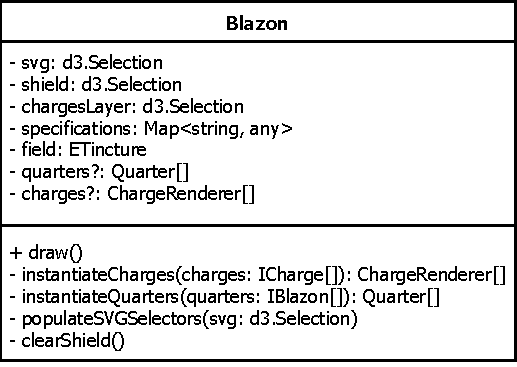
\includegraphics[width=0.5\linewidth]{BlazonUML}
  \caption{\texttt{Blazon} UML.}%
  \label{fig:BlazonUML}
\end{figure*}

\begin{figure*}[h]
  %\centering
  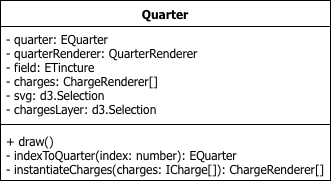
\includegraphics[width=0.5\linewidth]{QuarterUML}
  \caption{\texttt{Quarter} UML.}%
  \label{fig:QuarterUML}
\end{figure*}

\begin{figure*}[h]
  %\centering
  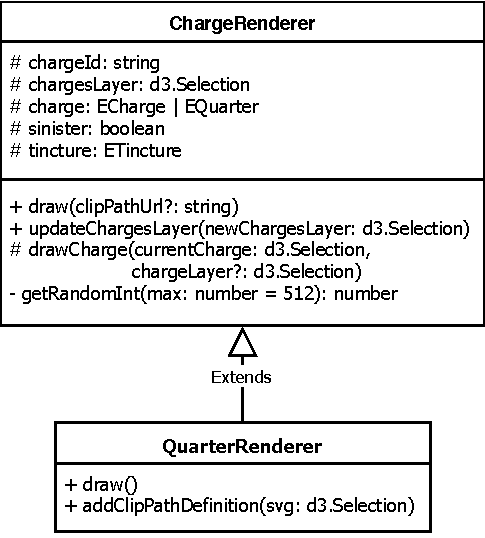
\includegraphics[width=0.5\linewidth]{ChargeRendererUML}%
  \caption{\texttt{ChargeRenderer} hierarchy and methods.}%
  \label{fig:charge_renderer_hierarchy}
\end{figure*}

\pagebreak%

\section{Third Design Iteration Diagrams}%
\label{sec:third_design_iteration_diagrams}

\begin{figure*}[h]
  %\centering
  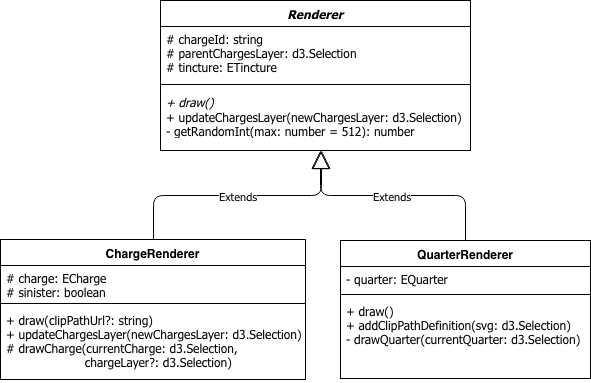
\includegraphics[width=0.8\linewidth]{RendererUML}
  \caption{\texttt{Renderer} hierarchy and methods.}%
  \label{fig:RendererUML}
\end{figure*}

\begin{figure*}[h]
  %\centering
  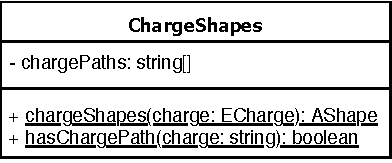
\includegraphics[width=0.5\linewidth]{ChargeShapesUML}
  \caption{\texttt{ChargeShapes} UML.}%
  \label{fig:ChargeShapesUML}
\end{figure*}

\begin{figure*}[h]
  %\centering
  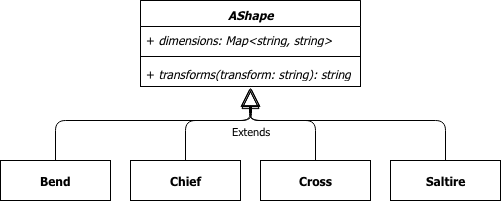
\includegraphics[width=0.8\linewidth]{AShapeUML}
  \caption{\texttt{AShape} hierarchy and methods.}%
  \label{fig:AShapeUML}
\end{figure*}

\setboolean{@mainmatter}{false}


\end{document}
